\documentclass[a4paper,fleqn]{cas-sc}

\usepackage[authoryear,longnamesfirst]{natbib}
\usepackage{lmodern}
\usepackage{microtype}
\usepackage{amsthm}
\usepackage{booktabs}
\usepackage{placeins}
\usepackage{needspace}
\IfFileExists{dsfont.sty}
  {\usepackage{dsfont}}
  {\let\mathds\mathbb}
\usepackage[nameinlink,capitalise]{cleveref}

\usepackage{nicefrac}



\newtheorem{theorem}{Theorem}
\newtheorem{lemma}{Lemma}
\newtheorem{proposition}{Proposition}
\newtheorem{corollary}{Corollary}
\theoremstyle{definition}
\newtheorem{definition}{Definition}
\theoremstyle{remark}
\newtheorem{remark}{Remark}

\newcommand{\R}{\mathds{R}}
\newcommand{\N}{\mathds{N}}
\newcommand{\Nzero}{\mathds{N}_0}
\newcommand{\Pp}{\mathds{P}}
\newcommand{\E}{\mathds{E}}
\newcommand{\norm}[1]{\left\lVert #1\right\rVert}
\newcommand{\set}[1]{\left\{#1\right\}}
\newcommand{\dd}{\,\mathrm{d}}
\newcommand{\Leb}{\lambda}
\newcommand{\ellpq}{\ell_{p,q}}
\newcommand{\upq}{u_{p,q}}
\newcommand{\kappaN}[1]{\kappa_{#1}}
\newcommand{\0}{\mathbf{0}}
\newcommand{\spherearea}[1]{\sigma_{#1}}
\ifdefined\SubmissionVersion
  \newcommand{\tr}[1]{#1}
  \newcommand{\tg}[1]{#1}
  \newcommand{\tb}[1]{#1}
  \newcommand{\tv}[1]{#1}
  \newcommand{\ttq}[1]{#1}
  \newcommand{\tor}[1]{#1}
  \newcommand{\tfg}[1]{#1}
  \newcommand{\tfr}[1]{#1}
  \newcommand{\tfb}[1]{#1}
  \newcommand{\ty}[1]{#1}
\else
  \newcommand{\tr}[1]{\textcolor[HTML]{aa0000}{#1}}
  \newcommand{\tg}[1]{\textcolor[HTML]{007700}{#1}}
  \newcommand{\tb}[1]{\textcolor[HTML]{0000bb}{#1}}
  \newcommand{\tv}[1]{\textcolor[HTML]{6A1B9A}{#1}}
  \newcommand{\ttq}[1]{\textcolor[HTML]{008B8B}{#1}}
  \newcommand{\tor}[1]{\textcolor[HTML]{C75B00}{#1}}
  \newcommand{\tfg}[1]{\textcolor[HTML]{00FF00}{#1}}
  \newcommand{\tfr}[1]{\textcolor[HTML]{FF0000}{#1}}
  \newcommand{\tfb}[1]{\textcolor[HTML]{666666}{#1}}
  \newcommand{\ty}[1]{\textcolor[HTML]{D4A900}{#1}}
\fi
\DeclareMathOperator{\SSG}{SSG}
\DeclareMathOperator{\BSG}{\beta SG}
\DeclareMathOperator{\RNG}{RNG}
\DeclareMathOperator{\GG}{GG}
\DeclareMathOperator{\Del}{Del}
\DeclareMathOperator{\MST}{MST}

\ExplSyntaxOn
\bool_gset_true:N \g_stm_nologo_bool
\ExplSyntaxOff


\emergencystretch=1em

\begin{document}
\let\WriteBookmarks\relax
\def\floatpagepagefraction{1}
\def\textpagefraction{.001}

\shorttitle{Structural Thresholds of Stepping-Stone Graphs}
\shortauthors{H. Espino-Montelongo and H. Maravillo}

\title[mode=title]{Structural Thresholds of Stepping-Stone Graphs
in Euclidean Space}

\author[1]{Heriberto Espino-Montelongo}
    [orcid=0009-0009-1230-2931]
\cormark[1]
\ead{heriberto.espinomo@udlap.mx}
\credit{
  Conceptualization,
  Methodology,
  Formal analysis,
  Investigation,
  Validation,
  Visualization,
  Writing -- original draft}

\affiliation[1]{
  organization={Universidad de las Am\'ericas Puebla},
  addressline={Ex Hacienda Santa Catarina M\'artir S/N},
  city={San Andr\'es Cholula},
  postcode={72810},
  state={Puebla},
  country={Mexico}
}

\author[2]{H\'ector Maravillo}
    [orcid=0000-0002-6101-1964]
\ead{hector.maravillo@uacm.edu.mx}
\credit{
  Investigation,
  Supervision,
  Visualization,
  Writing -- review and editing}

\affiliation[2]{
  organization={Universidad Aut\'onoma de la Ciudad de M\'exico},
  city={Ciudad de M\'exico},
  postcode={06720},
  country={Mexico}
}

\cortext[cor1]{Corresponding author}



\begin{abstract}
We study the structural properties of stepping-stone proximity graphs in
\(\R^d\), for every \(d\geq2\). The defining diversion neighborhoods form
a strictly increasing family between the segment, the Gabriel ball, and the
relative-neighborhood lune, so the associated graphs form an edge-decreasing
filtration. We derive dimension-independent inclusion chains with classical
proximity graphs and obtain two-sided comparisons with \(\beta\)-skeletons.
These comparisons recover the known planar Delaunay construction and transfer
connectivity, tiling-recovery, and spanning-ratio consequences.

The parameter \(\alpha=2\) is shown to be the sharp universal threshold, in
every ambient dimension, both for intersection-free straight-line
realizations and for containment in the Delaunay graph. Abstract planarity
behaves differently: \(\alpha=2\) is the sharp threshold in the plane,
whereas in every dimension \(d\geq3\) there are finite point sets whose
stepping-stone graph is nonplanar for every parameter. Finally, we extend the
planar stepping-stone spectrum to arbitrary dimension, give an exact
site-entry equation with the strict edge convention, bound the number of
distinct graphs in the filtration, and prove explicit finite-set
stabilization at the open relative-neighborhood graph. The construction is
available in Python through the open-source \textsc{ProximityGraphs} package.
\end{abstract}

\begin{keywords}
Stepping-stone graph \sep empty-region graph \sep proximity graph \sep
Delaunay graph \sep planarity \sep \(\beta\)-skeleton \sep graph filtration
\end{keywords}

\maketitle

\hypersetup{
  pdftitle={Structural Thresholds of Stepping-Stone Graphs in Euclidean Space},
  pdfauthor={Heriberto Espino-Montelongo and H\'ector Maravillo},
  pdfsubject={Structural Thresholds of Stepping-Stone Graphs in Euclidean Space},
  pdfkeywords={stepping-stone graph, empty-region graph, proximity graph, Delaunay graph, planarity, beta-skeleton, graph filtration}
}
\ifdefined\SubmissionVersion
  \hypersetup{hidelinks}
\fi

\section{Introduction}

An empty-region graph joins two sites whenever a region associated with the
pair contains no other site. The Gabriel graph, relative-neighborhood graph,
and \(\beta\)-skeletons are standard examples
\citep{gabriel1969statistical,toussaint1980relative,
jaromczyk1992relative,kirkpatrick1985framework}. Their structural properties
are controlled by the geometry and boundary convention of the corresponding
empty region. In the plane, \citet{cardinal2009empty} formalized this
dependence through convex and symmetric anchored regions and characterized
tight regions for several universal graph properties.

The stepping-stone graph was introduced by
\citet{kannangara2018stepping} and developed further by
\citet{kannangara2019stepping} for extracting movement corridors from sparse
trajectories. For distinct sites \(p,q\), its diversion neighborhood at
parameter \(\alpha\geq1\) consists of the points \(z\) satisfying
\begin{equation}
\norm{z-p}^{\alpha}+\norm{z-q}^{\alpha}
\leq \norm{p-q}^{\alpha}.
\end{equation}
The two sites are adjacent when this region contains no other point of the
input set. The original planar theory established graph monotonicity, the
Gabriel and relative-neighborhood endpoints, planarity for \(\alpha\geq2\),
a Delaunay-based construction, and the planar \(d\)-spectrum. The defining
Euclidean inequality, however, is meaningful in every ambient dimension.

This paper investigates the resulting structural theory in \(\R^d\).
The central distinction is between properties of a particular straight-line
realization and properties of the abstract graph. Two segments that intersect
properly always lie in a common affine plane, so a planar obstruction can
control geometric intersections in every dimension. Abstract planarity does
not behave this way: higher-dimensional point sets may realize nonplanar
graphs without any proper edge intersections.

Our first contribution is a dimension-independent region-inclusion analysis.
It yields the edge-decreasing stepping-stone filtration, its classical
proximity-graph chains, and explicit comparisons with both lune-based and
circle-based \(\beta\)-skeletons. These comparisons transfer connectivity,
Delaunay, tiling-recovery, and spanning-ratio results while keeping known
planar statements and their higher-dimensional extensions distinct.

Our second contribution is a sharp threshold theory. We prove that
\(\alpha=2\) is the exact universal threshold, in every dimension, for
intersection-free straight-line realizations and Delaunay containment. In the
plane it is also the exact threshold for abstract planarity. In dimensions at
least three, by contrast, finite integer-coordinate point sets produce
nonplanar stepping-stone graphs for every parameter.

Finally, we extend the stepping-stone spectrum of
\citet{kannangara2018stepping} to arbitrary dimension. An exact entry
equation determines when a site first enters a pair's diversion neighborhood.
For every finite point set, the resulting edge filtration changes only at
finitely many parameter values and stabilizes explicitly at the open
relative-neighborhood graph. The reusable construction is available in
Python through \textsc{ProximityGraphs}, complementing the earlier Java
implementation reported by Kannangara et al.

The remainder of the paper is organized as follows.
\Cref{sec:geometry} introduces the regions, boundary conventions, and
similarity normalization.
\Cref{sec:boundary-volume} records the endpoint and limiting regions.
\Cref{sec:monotonicity-graphs} develops the inclusion theory,
\(\beta\)-skeleton comparisons, sharp thresholds, dimension-dependent
planarity, and finite-set spectrum.
\Cref{sec:implementation} describes the available Java and Python
implementations.

\section{Definitions and geometric preliminaries}
\label{sec:geometry}

Throughout, \(d\geq2\) denotes the ambient dimension, and all points and
regions are considered in \(\R^d\). We write \(\0\) for the origin,
\(e_1\) for the first standard basis vector,
and
\begin{equation}
    B(x,r)
    :=
    \set{z\in\R^d:\norm{z-x}\leq r}
\end{equation}
for the closed Euclidean ball of radius $r$ centered at $x\in\R^d$, and
\begin{equation}
    B^\circ(x,r)
    :=
    \set{z\in\R^d:\norm{z-x}<r}
\end{equation}
for the corresponding open ball.
\begin{definition}[Stepping-stone diversion neighborhood]
Let $p,q\in\R^d$ be distinct, and set
\begin{equation}
    \ellpq:=\norm{q-p},
    \qquad
    \upq:=\frac{q-p}{\ellpq}.
\end{equation}
For $\alpha\geq1$, the stepping-stone diversion neighborhood determined by
$p$ and $q$ is
\begin{equation}\label{eq:ss-region}
    S_{\mathrm{SS},\alpha}(p,q)
    :=
    \set{
        z\in\R^d:
        \norm{z-p}^{\alpha}
        +
        \norm{z-q}^{\alpha}
        \leq
        \ellpq^{\alpha}
    }.
\end{equation}
Its normalized region is
\begin{equation}\label{eq:unit-region}
    K_{\mathrm{SS},\alpha}
    :=
    S_{\mathrm{SS},\alpha}(\0,e_1)
    =
    \set{
        z\in\R^d:
        \norm{z}^{\alpha}
        +
        \norm{z-e_1}^{\alpha}
        \leq1
    }.
\end{equation}
\end{definition}


\tv{For later comparison, the closed and open Gabriel regions determined by
$p$ and $q$ are the closed and open balls with diameter $pq$, respectively:}
\begin{equation}
    \tv{
    G_{\mathrm{cl}}(p,q)
    :=B\!\left(\frac{p+q}{2},\frac{\ellpq}{2}\right),
    \qquad
    G_{\mathrm{op}}(p,q)
    :=B^\circ\!\left(\frac{p+q}{2},\frac{\ellpq}{2}\right).
    }
\end{equation}
\tv{The closed and open relative-neighborhood lunes are, respectively,}
\begin{equation}
    L_{\mathrm{cl}}(p,q)
    :=B(p,\ellpq)\cap B(q,\ellpq),
    \qquad
    L_{\mathrm{op}}(p,q)
    :=B^\circ(p,\ellpq)\cap B^\circ(q,\ellpq).
\end{equation}
For a finite or locally finite set $V\subset\R^d$ and distinct $p,q\in V$,
these graphs are defined by
\begin{equation}
\begin{aligned}
pq\in E\bigl(\GG_{\mathrm{cl}}(V)\bigr)
&\iff
G_{\mathrm{cl}}(p,q)\cap\bigl(V\setminus\{p,q\}\bigr)=\varnothing,\\
pq\in E\bigl(\GG_{\mathrm{op}}(V)\bigr)
&\iff
G_{\mathrm{op}}(p,q)\cap\bigl(V\setminus\{p,q\}\bigr)=\varnothing,\\
pq\in E\bigl(\RNG_{\mathrm{cl}}(V)\bigr)
&\iff
L_{\mathrm{cl}}(p,q)\cap\bigl(V\setminus\{p,q\}\bigr)=\varnothing,\\
pq\in E\bigl(\RNG_{\mathrm{op}}(V)\bigr)
&\iff
L_{\mathrm{op}}(p,q)\cap\bigl(V\setminus\{p,q\}\bigr)=\varnothing.
\end{aligned}
\end{equation}
\tv{Thus $\GG_{\mathrm{cl}}(V)\subseteq\GG_{\mathrm{op}}(V)$ and
$\RNG_{\mathrm{cl}}(V)\subseteq\RNG_{\mathrm{op}}(V)$. Although the
corresponding region boundaries have zero $d$-dimensional volume, the graph
conventions may differ when a third site lies on such a boundary.}

\tv{Throughout the paper, $\GG(V)$ denotes $\GG_{\mathrm{cl}}(V)$ and
$\RNG(V)$ denotes $\RNG_{\mathrm{op}}(V)$, consistently with the original
stepping-stone construction and the empty-region conventions of
\citet{kannangara2018stepping,cardinal2009empty}. The alternative graphs
$\GG_{\mathrm{op}}(V)$ and $\RNG_{\mathrm{cl}}(V)$ are always identified
explicitly.}

\begin{definition}[Stepping-stone graph]
For a finite or locally finite set $V\subset\R^d$, the stepping-stone
graph with parameter $\alpha$ is the graph
\tv{$\SSG_\alpha(V)=(V,E_\alpha(V))$} such that two distinct points
$p,q\in V$ are adjacent if
\begin{equation}
    S_{\mathrm{SS},\alpha}(p,q)
    \cap
    \bigl(V\setminus\{p,q\}\bigr)
    =
    \emptyset.
\end{equation}
\end{definition}

\begin{proposition}[Similarity normalization]
\label{prop:factorization}
If $Q$ is an orthogonal transformation satisfying $Qe_1=\upq$, then
\begin{equation}\label{eq:similarity-normalization}
    S_{\mathrm{SS},\alpha}(p,q)
    =
    p+\ellpq QK_{\mathrm{SS},\alpha}.
\end{equation}
The right-hand side is independent of the chosen transformation $Q$.
\end{proposition}

\begin{proof}
For $w\in\R^d$, substitute $z=p+\ellpq Qw$ in
\eqref{eq:ss-region}. The two normalized distances become $\norm{w}$ and
$\norm{w-e_1}$, proving \eqref{eq:similarity-normalization}. If $Q_1$ and
$Q_2$ both send $e_1$ to $\upq$, then $Q_2^{-1}Q_1$ fixes $e_1$. The
normalized region is invariant under every such orthogonal transformation,
so $Q_1K_{\mathrm{SS},\alpha}=Q_2K_{\mathrm{SS},\alpha}$.
\end{proof}

Thus it suffices to study the normalized region
$K_{\mathrm{SS},\alpha}$. \Cref{fig:ss-regions} shows the same three
\tv{representative} parameter values in two and three dimensions. The dashed planar
boundary is the limiting relative-neighborhood lune.

\begin{figure}[pos=tb]
    \centering
    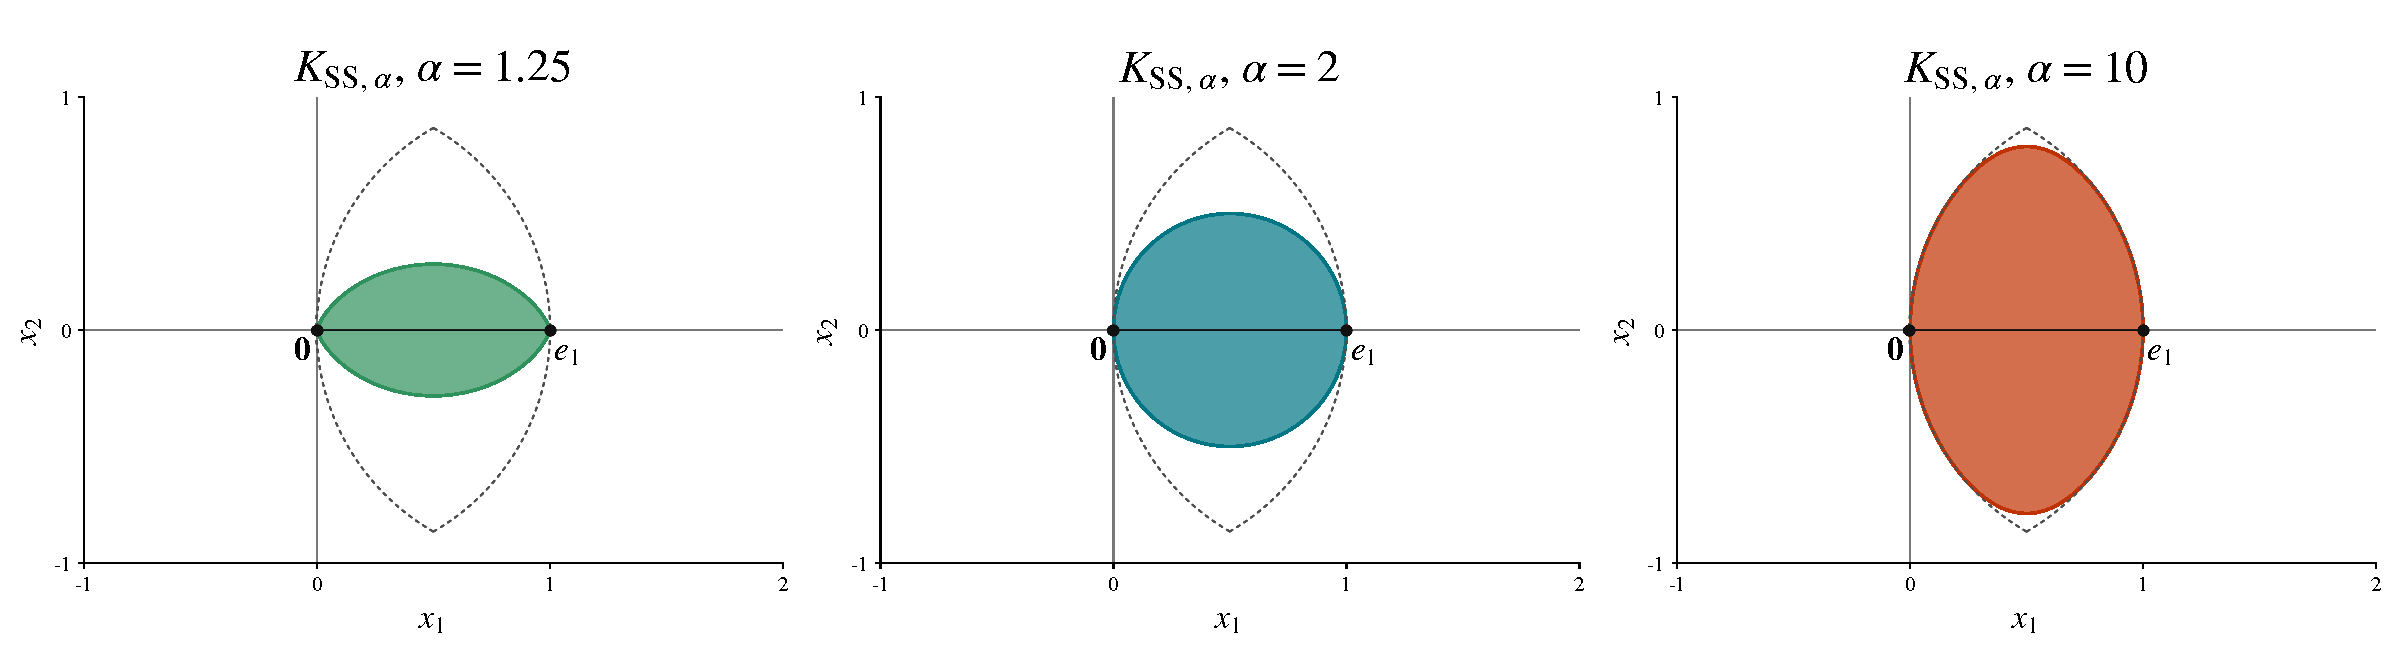
\includegraphics[width=0.98\linewidth]{stepping_stone_region_templates.pdf}
    \vspace{3pt}

    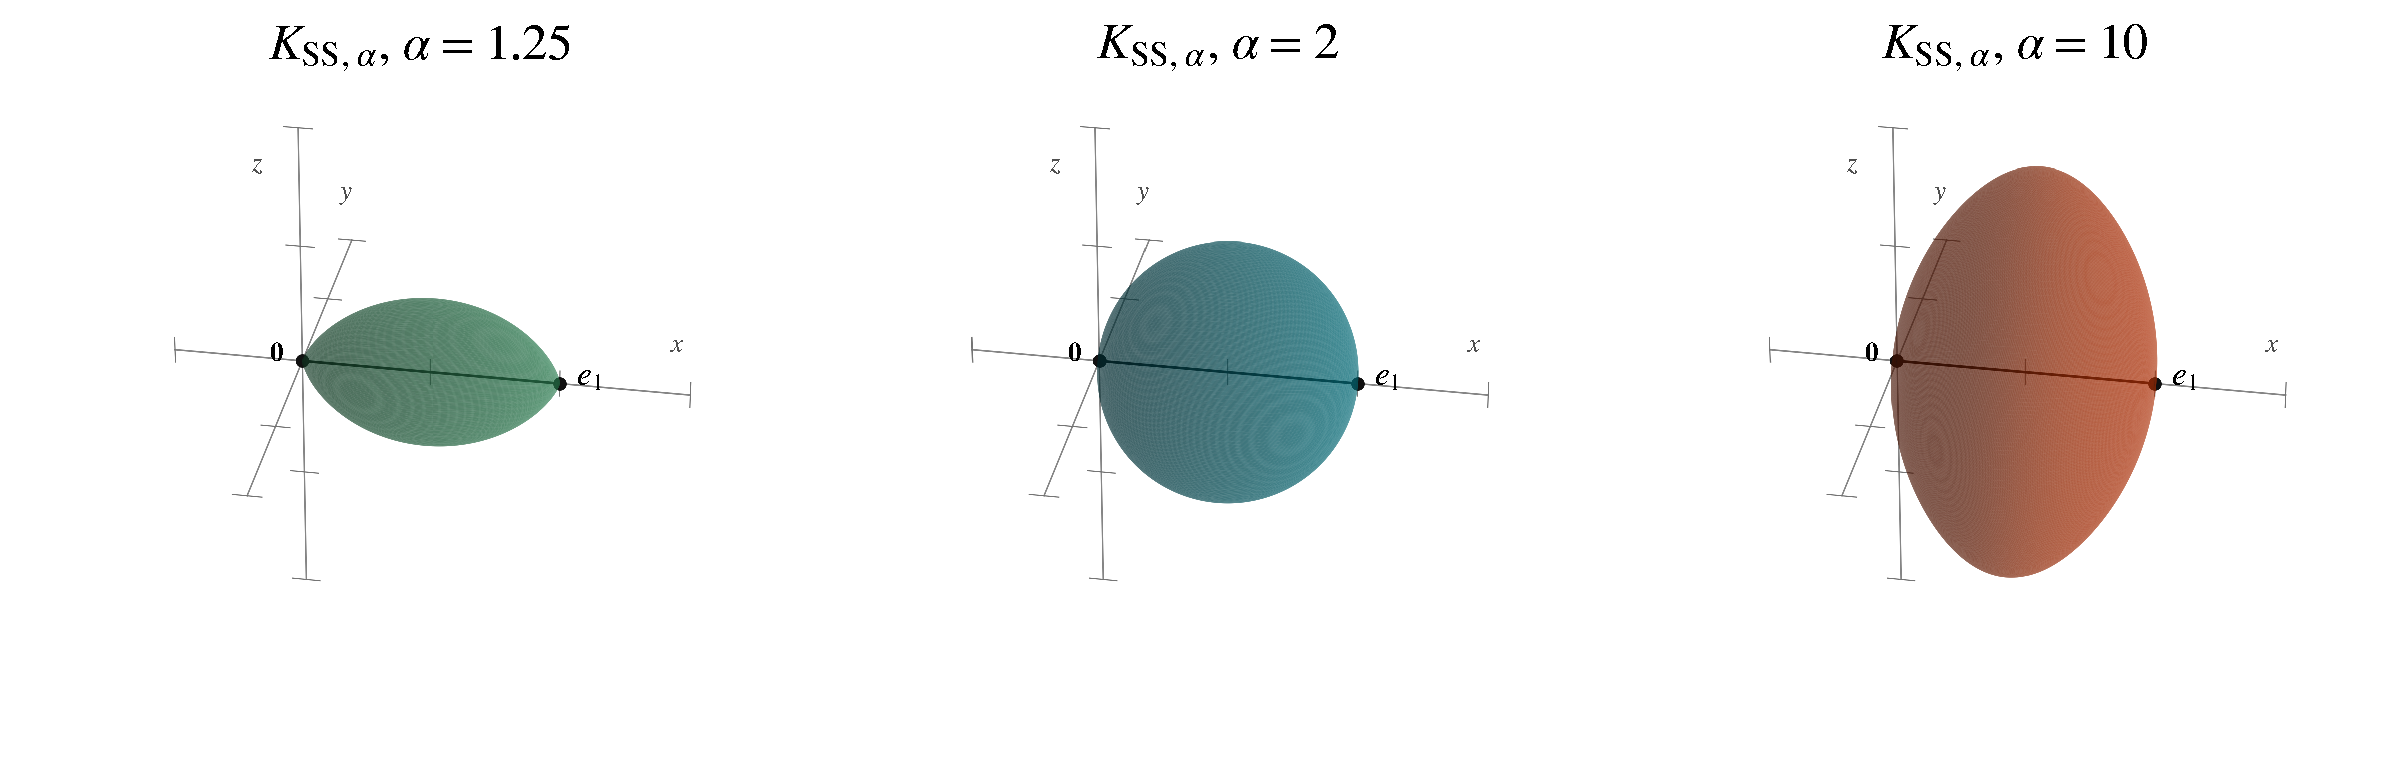
\includegraphics[width=0.98\linewidth]{stepping_stone_three_dimensional_regions.pdf}
    \caption{Normalized stepping-stone diversion neighborhoods for
    $\alpha=1.25$, $2$, and $10$. Top: planar regions, with the limiting
    relative-neighborhood lune shown by the dashed boundary. Bottom:
    three-dimensional regions for the same parameter values. The defining
    sites are fixed at $\0$ and $e_1$.}
    \label{fig:ss-regions}
\end{figure}
\FloatBarrier

To complement the static views in \Cref{fig:ss-regions}, the computational
companion~\citep{espino2026computational} provides an
\href{https://heri-espino.github.io/Stepping-Stone-Volume-Constants/}
{interactive three-dimensional visualization} of the normalized diversion
neighborhood. 

\begin{proposition}[Elementary geometry]\label{prop:geometry}
For every $\alpha\geq1$, the region $S_{\mathrm{SS},\alpha}(p,q)$ is compact
and convex. It is centrally symmetric about
\begin{equation}
    m:=\frac{p+q}{2}
\end{equation}
and \ttq{invariant under every Euclidean isometry fixing the line through
$p$ and $q$ pointwise}. If $\alpha>1$, then
$S_{\mathrm{SS},\alpha}(p,q)$ has nonempty interior and is strictly convex.
\end{proposition}

\begin{proof}
The function
\begin{equation}
    F_{p,q,\alpha}(z)
    :=\norm{z-p}^{\alpha}+\norm{z-q}^{\alpha}
\end{equation}
is continuous and convex for $\alpha\geq1$. Hence its sublevel set
$S_{\mathrm{SS},\alpha}(p,q)$ is closed and convex. Its defining inequality
implies
\begin{equation}
    \norm{z-p}\leq\ellpq,
    \qquad
    \norm{z-q}\leq\ellpq,
\end{equation}
so the region is bounded and therefore compact.

The reflection $z\mapsto p+q-z$ exchanges the two distance terms and preserves
the region, proving central symmetry. \ttq{Every Euclidean isometry fixing
the line through $p$ and $q$ pointwise preserves both distances} and
therefore preserves the region.

For $\alpha>1$, the map $z\mapsto\norm{z-p}^{\alpha}$ is strictly convex, and
so is $F_{p,q,\alpha}$. If $z_1\neq z_2$ belong to the region and
$t\in(0,1)$, then
\begin{equation}
    F_{p,q,\alpha}\left(tz_1+(1-t)z_2\right)
    <tF_{p,q,\alpha}(z_1)+(1-t)F_{p,q,\alpha}(z_2)
    \leq\ellpq^{\alpha}.
\end{equation}
Thus the open segment joining $z_1$ and $z_2$ lies in the interior. Moreover,
\begin{equation}
    F_{p,q,\alpha}(m)
    =2\left(\frac{\ellpq}{2}\right)^{\alpha}
    =2^{1-\alpha}\ellpq^{\alpha}
    <\ellpq^{\alpha},
\end{equation}
so the interior is nonempty.
\end{proof}


\section{Endpoint and limiting regions}
\label{sec:boundary-volume}

The stepping-stone family interpolates between three classical regions. We
record the endpoint identities and the precise relative-neighborhood limit
before studying the resulting graph filtration. All statements hold in every
ambient dimension \(d\geq2\).

The graph identity at \(\alpha=2\) was established in the original
planar stepping-stone study by
\citet[Theorem~3.4]{kannangara2018stepping}. The following formulation keeps
the boundary convention explicit and holds in every dimension.

\begin{proposition}[Segment and Gabriel endpoints]
\label{prop:special-cases}
At \(\alpha=1\), the diversion neighborhood is the segment \([p,q]\).
At \(\alpha=2\), it is the closed ball with diameter \(pq\). Consequently,
\(\SSG_2(V)=\GG(V)\) for every finite or locally finite point set \(V\).
At \(\alpha=1\), two sites are adjacent precisely when the open segment
joining them contains no other site; hence \(\SSG_1(V)\) is complete
whenever no three sites are collinear.
\end{proposition}

\begin{proof}
At \(\alpha=1\), the triangle inequality is an equality precisely on the
segment joining \(p\) and \(q\). At \(\alpha=2\), put
\(m=(p+q)/2\). The parallelogram identity gives
\begin{equation}
\norm{z-p}^2+\norm{z-q}^2
=
2\norm{z-m}^2+2\left(\frac{\ellpq}{2}\right)^2,
\end{equation}
so the defining inequality is equivalent to
\(\norm{z-m}\leq\ellpq/2\). The graph statements follow from deleting
the defining sites and from the closed Gabriel-ball convention.
\end{proof}


The convergence of the planar graph to the relative-neighborhood graph was
identified by \citet[Theorem~3.5]{kannangara2018stepping}. The next result
states the corresponding region limit in arbitrary dimension.

\begin{proposition}[Convergence to the relative-neighborhood lune]
\label{prop:rng-limit}
The diversion neighborhoods increase from within to the open
relative-neighborhood lune:
\begin{equation}\label{eq:open-lune-limit}
\bigcup_{1<\alpha<\infty}
\left(S_{\mathrm{SS},\alpha}(p,q)\setminus\{p,q\}\right)
=
L_{\mathrm{op}}(p,q).
\end{equation}
\end{proposition}

\begin{proof}
For \(z\notin\{p,q\}\), the defining inequality implies
\begin{equation}
\norm{z-p}<\ellpq,
\qquad
\norm{z-q}<\ellpq.
\end{equation}
Thus every finite-parameter diversion neighborhood, after removal of its
defining sites, is contained in \(L_{\mathrm{op}}(p,q)\).

Conversely, if \(z\in L_{\mathrm{op}}(p,q)\), then both normalized
distances
\begin{equation}
\frac{\norm{z-p}}{\ellpq},
\qquad
\frac{\norm{z-q}}{\ellpq}
\end{equation}
are strictly smaller than one. The sum of their \(\alpha\)th powers tends
to zero as \(\alpha\to\infty\), so \(z\) belongs to the diversion
neighborhood for every sufficiently large \(\alpha\).
\end{proof}


\section{Monotonicity and graph consequences}
\label{sec:monotonicity-graphs}

The region inclusion chains, connectivity, and spectrum formulation below
hold in every ambient dimension. The intersection and Delaunay thresholds
also hold in every dimension, while the candidate-count, tiling, dilation,
and abstract-planarity statements identified as planar remain restricted to
\(\R^2\).

\subsection{Strict region monotonicity}

The edge monotonicity of the original planar family is due to
\citet[Theorem~3.3]{kannangara2018stepping}. We first record the strict
region refinement used throughout the paper.

\begin{theorem}[Strict region monotonicity]
\label{thm:monotonicity}
For every \(1\leq\alpha_1<\alpha_2\) and every distinct
\(p,q\in\R^d\),
\begin{equation}
S_{\mathrm{SS},\alpha_1}(p,q)
\subsetneq
S_{\mathrm{SS},\alpha_2}(p,q).
\end{equation}
\end{theorem}

\begin{proof}
For \(a,b\geq0\), the map
\begin{equation}
r\longmapsto\left(a^r+b^r\right)^{1/r},
\qquad r>0,
\end{equation}
is nonincreasing. Applying this fact to
\(a=\norm{z-p}\) and \(b=\norm{z-q}\) proves the non-strict inclusion.

For strictness, let \(m=(p+q)/2\) and choose a unit vector \(v\)
perpendicular to \(q-p\). A point \(m+tv\) belongs to
\(S_{\mathrm{SS},\alpha}(p,q)\) precisely when
\begin{equation}
|t|
\leq
\ellpq\sqrt{2^{-2/\alpha}-\frac14}.
\end{equation}
The right-hand side is strictly increasing in \(\alpha\). Choosing \(t\)
strictly between the radii corresponding to \(\alpha_1\) and
\(\alpha_2\) gives a point in the larger region but not in the smaller.
\end{proof}

\subsection{Monotonicity and graph inclusions}
\label{sec:inclusions}

The following order principle applies beyond the stepping-stone
family. Let \(K\subset\R^d\) contain the anchors \(\0,e_1\) and be
invariant under every orthogonal transformation fixing \(e_1\). For
distinct \(p,q\), define its pairwise unit-region image by
\begin{equation}
S_K(p,q):=p+\ellpq Q_{p,q}K,
\qquad
Q_{p,q}e_1=\upq.
\end{equation}
The invariance condition makes this definition independent of the chosen
orthogonal transformation. It is the natural arbitrary-dimensional analogue
of the anchored-template construction of \citet{cardinal2009empty} for this
axially symmetric setting.

Let \(G_K(V)\) join \(p\) and \(q\) precisely when \(S_K(p,q)\)
contains no site of \(V\setminus\{p,q\}\). For any two such templates,
region inclusion reverses edge inclusion:
\begin{equation}\label{eq:unit-region-order-reversal}
K_1\setminus\{\0,e_1\}
\subseteq
K_2\setminus\{\0,e_1\}
\quad\Longrightarrow\quad
G_{K_2}(V)\subseteq G_{K_1}(V).
\end{equation}
Indeed, an empty copy of the larger region has an empty copy of the smaller
region. The rest of the paper applies this elementary transfer principle to
the nested templates \(K_{\mathrm{SS},\alpha}\).

\tv{Let $\MST(V)$ denote a Euclidean minimum spanning tree of a
\ttq{nonempty} finite point set $V$, and let $\Del(V)$ denote its Delaunay graph
\citep{mitchell2018}. With the closed Gabriel-ball and open
relative-neighborhood-lune conventions adopted above, the standard
inclusions are}
\begin{equation}
    \tv{
    \MST(V)\subseteq\RNG(V)\subseteq\GG(V)\subseteq\Del(V).
    }
\end{equation}
\tv{The hierarchy is reviewed by \citet{jaromczyk1992relative}; the
closed-ball Gabriel convention and its Delaunay inclusion are explicit in
\citet[Lemmas~1--2]{matula1980properties} and
\citet{cardinal2009empty}. In particular, an empty closed diametral ball
itself certifies the Delaunay empty-ball condition, including configurations
with cospherical sites.}
\tfg{In the planar setting, the graph nesting, the Gabriel and
relative-neighborhood endpoints, and the Delaunay containment for parameters
at least two were established by
\citet[Theorems~3.3--3.5 and~3.11]{kannangara2018stepping}. The next
proposition gives a region-based derivation that makes the open--closed
conventions explicit and extends the resulting inclusion chains to every
ambient dimension.}

\begin{proposition}[Monotonicity and classical proximity-graph inclusions]
\label{prop:inclusions}
If $1\leq\alpha_1<\alpha_2$, then
\begin{equation}\label{eq:ss-edge-monotonicity}
    E_{\alpha_2}(V)\subseteq E_{\alpha_1}(V).
\end{equation}
Thus $\{\SSG_\alpha(V):\alpha\geq1\}$ is a monotonically decreasing family
of graphs under edge inclusion, although the inclusion need not be strict for
a fixed point set.
Furthermore, for every \ttq{nonempty} finite $V\subset\R^d$ and every finite
$\alpha\geq1$,
\begin{equation}
    \MST(V)\subseteq\RNG(V)\subseteq\SSG_\alpha(V).
\end{equation}
If $1\leq\alpha\leq2$, then
\begin{equation}
    \MST(V)\subseteq\RNG(V)\subseteq\GG(V)
    \subseteq\SSG_\alpha(V).
\end{equation}
If $\alpha\geq2$, then
\begin{equation}\label{eq:tail-chain}
    \MST(V)\subseteq\RNG(V)\subseteq\SSG_\alpha(V)
    \subseteq\GG(V)\subseteq\Del(V).
\end{equation}
\end{proposition}

\begin{proof}
The first edge inclusion follows directly from \Cref{thm:monotonicity} and
the preceding implication; it is the region-inclusion formulation of the
nestedness proved for the original $d$-spectrum by
\citet{kannangara2018stepping,kannangara2019stepping}.

For $z\notin\{p,q\}$, the inequality defining
$S_{\mathrm{SS},\alpha}(p,q)$ implies
\begin{equation}
    \norm{z-p}<\ellpq,
    \qquad
    \norm{z-q}<\ellpq.
\end{equation}
Thus
$S_{\mathrm{SS},\alpha}(p,q)\setminus\{p,q\}
\subset L_{\mathrm{op}}(p,q)$,
and the same implication gives $\RNG(V)\subseteq\SSG_\alpha(V)$. The remaining
stepping-stone inclusions follow from
\Cref{prop:special-cases,thm:monotonicity}; the other inclusions are
classical.
\end{proof}

\clearpage
\begingroup

% Keep these local redefinitions within the present group.
\renewcommand{\tr}[1]{#1}
\renewcommand{\tg}[1]{#1}
\renewcommand{\tb}[1]{#1}
\renewcommand{\tv}[1]{#1}
\renewcommand{\tor}[1]{#1}
\renewcommand{\ttq}[1]{#1}
\renewcommand{\tfg}[1]{#1}
\renewcommand{\tfr}[1]{#1}
\renewcommand{\tfb}[1]{#1}

Following the standard terminology of
\citet[Sec.~II-C]{jaromczyk1992relative} and
\citet[Sec.~2]{eppstein2002beta}, and the planar lune-based formulation of
\citet[Def.~1]{maravillo2023cyclic}, let $N_\beta(p,q)$ denote the closed
region of influence of the $\beta$-skeleton. We use the closed-region
convention throughout, so that the treatment of sites on the boundary is
explicit. For
$1\leq\beta\leq2$, the lune-based region is the intersection of the two
closed balls of radius $\beta\ellpq/2$ centered at
\begin{equation}
    c_1=p+\frac{\beta}{2}(q-p),
    \qquad
    c_2=q+\frac{\beta}{2}(p-q).
\end{equation}
For $0<\beta\leq1$, the circle-based region is the intersection of the
two closed disks of radius $\ellpq/(2\beta)$ whose boundaries contain
$p$ and $q$.  The two definitions agree at $\beta=1$.  At $\beta=0$,
we use the limiting region $N_0(p,q)=[p,q]$.  The corresponding
$\beta$-skeleton is denoted by $\BSG_\beta(V)$ and is defined by
\begin{equation}\label{eq:beta-skeleton-definition}
    pq\in E\bigl(\BSG_\beta(V)\bigr)
    \quad\Longleftrightarrow\quad
    N_\beta(p,q)\cap\bigl(V\setminus\{p,q\}\bigr)=\varnothing.
\end{equation}
Thus $\BSG_1(V)=\GG(V)$, while the lune-based $2$-skeleton is the
relative-neighborhood graph. The same endpoint terminology is used by
\citet[Def.~1]{maravillo2023cyclic}; our closed-region convention fixes the
treatment of boundary sites as specified above.

\begin{proposition}[Comparison with $\beta$-skeletons]
\label{prop:beta-comparison}
For $\alpha\geq2$, set
\begin{equation}\label{eq:beta-plus}
    \beta_+(\alpha):=2^{\,1-2/\alpha}\in[1,2).
\end{equation}
Then, for every finite $V\subset\R^d$,
\begin{equation}\label{eq:beta-upper-chain}
    \RNG(V)
    \subseteq \SSG_\alpha(V)
    \subseteq \BSG_{\beta_+(\alpha)}(V)
    \subseteq \GG(V)
    \subseteq \Del(V).
\end{equation}

For $1\leq\alpha\leq2$, define
\begin{equation}\label{eq:beta-minus}
    \rho_\alpha
    :=\sqrt{2^{-2/\alpha}-\frac14},
    \qquad
    \beta_-(\alpha)
    :=\frac{4\rho_\alpha}{1+4\rho_\alpha^2}\in[0,1].
\end{equation}
Then, for every finite planar point set $V\subset\R^2$,
\begin{equation}\label{eq:beta-lower-chain}
    \GG(V)
    \subseteq \SSG_\alpha(V)
    \subseteq \BSG_{\beta_-(\alpha)}(V).
\end{equation}
The endpoint values are
\begin{equation}
    \beta_-(1)=0,
    \qquad
    \beta_-(2)=\beta_+(2)=1.
\end{equation}
For each fixed $\alpha$, these values are best possible: in the respective
parameter range, $\beta_-(\alpha)$ or $\beta_+(\alpha)$ is the largest
$\beta$ for which
\begin{equation}\label{eq:beta-region-comparison}
    N_\beta(p,q)\subseteq S_{\mathrm{SS},\alpha}(p,q)
\end{equation}
holds for every pair $p,q$.
\end{proposition}

\begin{proof}
For $\alpha\geq2$, the planar comparison with the lune-based
$\beta$-skeleton is due to
\citet[Theorem~3.10]{kannangara2018stepping}.  The same calculation applies
in $\R^d$.  Normalize $p=\0$ and $q=e_1$, write
$z=(x,Z)$ with $r=\norm{Z}$, and put $a=\alpha/2\geq1$.  By symmetry it is
enough to take $0\leq x\leq1/2$.  On the boundary of the lune-based
region of influence $N_\beta(\0,e_1)$,
\begin{equation}
    r^2=\beta x-x^2.
\end{equation}
Consequently, on that boundary the left-hand side of the normalized
stepping-stone inequality is
\begin{equation}
    f(x)
    :=(\beta x)^a+\bigl(1-(2-\beta)x\bigr)^a.
\end{equation}
For $\beta=\beta_+(\alpha)$, the convex function $f$ has
$f(0)=f(1/2)=1$, and therefore $f(x)\leq1$ on $[0,1/2]$.  Hence
$N_{\beta_+(\alpha)}(\0,e_1)$ is contained in the stepping-stone region.
Therefore, if the stepping-stone region contains no site of
$V\setminus\{p,q\}$, neither does $N_{\beta_+(\alpha)}(p,q)$, which proves
the middle inclusion in \eqref{eq:beta-upper-chain}.  The remaining
inclusions follow from \Cref{prop:inclusions} and the monotonicity of
$\beta$-skeletons: as $\beta$ increases, the region of influence expands
and the graph becomes sparser
\citep[Observation~1]{bose2006spanning}.

Now let $1<\alpha<2$ and consider a boundary point $z$ of the normalized
stepping-stone region.  Put
\begin{equation}
    u:=\norm{z}^{\alpha},
    \qquad
    1-u:=\norm{z-e_1}^{\alpha},
    \qquad
    b:=\frac{2}{\alpha}\in(1,2).
\end{equation}
If $\theta=\angle \0 z e_1$, the cosine law gives
\begin{equation}
    \cos\theta
    =
    \frac{u^b+(1-u)^b-1}
         {2\{u(1-u)\}^{b/2}}.
\end{equation}
A direct differentiation shows that this symmetric expression is minimized
at $u=1/2$.  Thus the largest boundary angle occurs in the midpoint slice
and satisfies
\begin{equation}
    \cos\theta_\alpha
    =1-2^{\,2/\alpha-1},
    \qquad
    \sin\theta_\alpha=\beta_-(\alpha).
\end{equation}
By the angle definition of the circle-based $\beta$-skeleton
\citep[Sec.~2]{eppstein2002beta}, its region of influence is
\begin{equation}
    \set{z:\angle pzq\geq
    \pi-\arcsin\bigl(\beta_-(\alpha)\bigr)}.
\end{equation}
To prove the containment, suppose that a point of this region
were outside the stepping-stone region.  Its longitudinal coordinate lies
between those of $p$ and $q$.  Moving transversely toward $[p,q]$ at that
fixed coordinate must first meet the stepping-stone boundary.  The subtended
angle strictly increases during this motion, producing a boundary angle
larger than $\theta_\alpha$, contrary to the preceding maximum.  Thus
$N_{\beta_-(\alpha)}(p,q)$ is contained in the stepping-stone region.
The edge inclusion follows again from the definition of an empty-region
graph, and the first inclusion in \eqref{eq:beta-lower-chain} follows from
\Cref{prop:inclusions}.  The endpoint cases $\alpha=1,2$ follow from the
segment and closed Gabriel-ball cases.

It remains to prove that the parameters are best possible.  In the
hyperplane through the midpoint and perpendicular to $pq$, the maximum
distance from the line $pq$ is $\rho_\alpha$ for the stepping-stone region.
The definitions of $\beta_-(\alpha)$ and $\beta_+(\alpha)$ make the
corresponding region of influence reach exactly this distance.  This
distance is strictly increasing with $\beta$ for both the circle-based and
lune-based definitions.  Hence every larger $\beta$ gives a point of
$N_\beta(p,q)$ outside the stepping-stone region, so
\eqref{eq:beta-region-comparison} fails.
\end{proof}

\begin{remark}[Parameter values and consequences of inclusion]
For example,
\begin{equation}
    \beta_-(1.25)\approx0.8568,
    \qquad
    \beta_-(1.5)\approx0.9656,
    \qquad
    \beta_-(1.75)\approx0.9946.
\end{equation}
Every graph property closed under taking subgraphs passes from
$\BSG_{\beta_+(\alpha)}(V)$ to $\SSG_\alpha(V)$, and deleting edges cannot
decrease shortest-path distances.  The inclusions alone do not imply
connectivity or an upper bound on the spanning ratio, and the fact that a
supergraph is dense or nonplanar gives no such conclusion for its
subgraphs.  Connectivity follows separately from
$\MST(V)\subseteq\SSG_\alpha(V)$.
\end{remark}

\begin{corollary}[Planar embedding and Delaunay containment]
\label{cor:beta-planar-structure}
Let $V\subset\R^2$ be finite with $n:=|V|\geq3$, and let
$\alpha\geq2$.  Then the geometric realization of
$\SSG_\alpha(V)$ is planar, and $\SSG_\alpha(V)$ is a subgraph of the
Delaunay graph.  In particular, it has at most $3n-6$ edges and is
four-colorable.
\end{corollary}

\begin{proof}
For $1\leq\beta\leq2$, the lune-based $\beta$-skeleton is planar and is a
subgraph of the Delaunay graph
\citep{jaromczyk1992relative,maravillo2023cyclic}.  The conclusion follows
from \eqref{eq:beta-upper-chain} because planarity and Delaunay containment
are preserved under taking subgraphs.  The edge bound and four-colorability
are standard consequences of planarity.
\end{proof}

\begin{corollary}[Cyclic tilings]
\label{cor:cyclic-tiling}
Let $\mathcal T=\{T_1,T_2,\ldots\}$ be a cyclic tiling of the plane, with
discrete vertex set $V_{\mathcal T}$ and edge set $E_{\mathcal T}$.  The
empty-region definition extends without change from finite point sets to
discrete point sets.  For every finite $\alpha\geq2$,
\begin{equation}
    E\bigl(\SSG_\alpha(V_{\mathcal T})\bigr)
    \subseteq E_{\mathcal T}.
\end{equation}
Thus every edge of the stepping-stone graph is an edge of the tiling.
\end{corollary}

\begin{proof}
For $\alpha\geq2$, \Cref{prop:beta-comparison} gives
\begin{equation}
    \SSG_\alpha(V_{\mathcal T})
    \subseteq \BSG_{\beta_+(\alpha)}(V_{\mathcal T}),
    \qquad
    1\leq\beta_+(\alpha)<2.
\end{equation}
By \citet[Theorem~1]{maravillo2023cyclic}, if
$\BSG_{\beta_+(\alpha)}(V_{\mathcal T})=(V_{\mathcal T},E_\beta)$, then
$E_\beta\subseteq E_{\mathcal T}$.  The result follows by transitivity.
\end{proof}

\clearpage

\begin{remark}[\tfg{Delaunay starting graph in the plane}]
\label{rem:delaunay-candidates}
\tfg{For $\alpha\geq2$, \citet[Theorem~3.11 and Algorithm~1]
{kannangara2018stepping} use the Delaunay triangulation as the starting
graph for computing the planar $d$-spectrum.  In the notation used here,
let $V\subset\R^2$ be a finite point set in
Delaunay general position (no three sites collinear and no four sites
cocircular), let $n=|V|\geq3$, and let $\alpha\geq2$. By
\eqref{eq:tail-chain}, every edge of $\SSG_\alpha(V)$ is an edge of
$\Del(V)$. Hence at most $3n-6$ Delaunay edges need to be examined.  The
naive algorithm that compares every such edge with the remaining $n-2$
sites takes $O(n^2)$ time; the linear number of Delaunay edges alone does
not give a linear-time algorithm.  For comparison,
\citet{lingas1994linear} construct the planar RNG and lune-based
$\beta$-skeletons from the Delaunay triangulation, while proximity
algorithms in higher dimensions require different methods
\citep{dickerson1996algorithms}.}
\end{remark}

\begin{remark}[\tr{Higher-dimensional Delaunay consequences}]
\tr{For $\alpha\geq2$, \Cref{prop:inclusions} places
$\SSG_\alpha(V)$ inside the Delaunay graph in every dimension. Therefore,
every graph property closed under taking subgraphs passes from
$\Del(V)$ to $\SSG_\alpha(V)$. In particular, the shallow-minor bounds
proved by \citet{teng1998combinatorial} for Delaunay diagrams of random
point sets also hold for the stepping-stone graph under the same random
point model.  This containment does not imply a linear number of edges in
higher dimensions: Delaunay graphs can have $\Theta(n^2)$ edges in
$\R^3$ \citep{agarwal1992relative}, and the maximum number of edges in a
Gabriel graph is also $\Theta(n^2)$ in dimension three and higher
\citep[Lemma~5.1]{chazelle1994selecting}.}
\end{remark}

\begin{corollary}[\tfg{Connectivity and planar geometric realization}]
\label{cor:ss-connectivity}
\tfg{For every nonempty finite $V\subset\R^d$ and every finite
$\alpha\geq1$, the graph $\SSG_\alpha(V)$ is connected. If
$V\subset\R^2$ and $\alpha\geq2$, its geometric realization is planar.}
\end{corollary}

\begin{proof}
\tfg{The planar statements correspond to
\citet[Lemmas~3.6--3.8]{kannangara2018stepping}. The
connectivity assertion in arbitrary dimension follows because the graph
contains a Euclidean minimum spanning tree for every finite
$\alpha\geq1$. If $V\subset\R^2$ and $\alpha\geq2$, then
$\SSG_\alpha(V)\subseteq\GG(V)$ by \eqref{eq:tail-chain}, and the planar
Gabriel graph has a planar geometric realization.}
\end{proof}

\tr{For a connected geometric graph $G$ on $V\subset\R^2$, write
$d_G(p,q)$ for the Euclidean length of a shortest path from $p$ to $q$ in
$G$.  Its spanning ratio, also called its dilation, is}
\begin{equation}\label{eq:dilation}
\tr{
\operatorname{dil}(G)
:=
\max_{p\ne q\in V}
\frac{d_G(p,q)}{\norm{p-q}}.
}
\end{equation}
\tr{Equivalently, $G$ is a geometric $t$-spanner when
$\operatorname{dil}(G)\leq t$
\citep{cardinal2009empty,bose2013spanners}.}

\clearpage

\begin{corollary}[\tfg{Unbounded spanning ratio}]
\label{cor:unbounded-dilation}
\tfg{For every fixed $\alpha>1$ and every $T>0$, there exists a finite
point set $V\subset\R^2$ such that $\SSG_\alpha(V)$ is connected and}
\begin{equation}
\tfg{
\operatorname{dil}\bigl(\SSG_\alpha(V)\bigr)>T.
}
\end{equation}
\tfg{If $\alpha\geq2$, its geometric realization is planar. Thus no fixed
$\alpha>1$ makes the stepping-stone graph a geometric $t$-spanner for all
planar point sets, for any constant $t$.}
\tfg{The restriction $\alpha>1$ is essential: at $\alpha=1$, every planar
point set in general position yields the complete graph and hence dilation
one.}
\end{corollary}

\begin{proof}
\tfg{For every $\alpha>1$, \Cref{prop:geometry} shows that the normalized
stepping-stone template is convex and symmetric and has nonempty interior.
Therefore \citet[Theorem~13]{cardinal2009empty} applies: for every anchored
region with nonempty interior, they construct planar point sets whose
spanning ratio is $\Omega(n^c)$ for some $c>0$.
Connectivity follows from \Cref{cor:ss-connectivity}; the same corollary
gives a planar geometric realization when $\alpha\geq2$.
For this latter range, the conclusion can alternatively be obtained from
the unbounded dilation of Gabriel graphs proved by
\citet{eppstein2002beta}, because $\SSG_\alpha(V)$ is a connected subgraph
of $\GG(V)$.}
\end{proof}

\begin{corollary}[Lower bounds on the spanning ratio]
\label{cor:quantitative-dilation}
The qualitative conclusion of \Cref{cor:unbounded-dilation} admits the
following quantitative refinements.
\begin{enumerate}
\item[(i)] For every fixed finite $\alpha\geq2$ and every $n\geq2$, there
exists a set $V_n$ of $n$ points in the plane such that
\begin{equation}
    \operatorname{dil}\bigl(\SSG_\alpha(V_n)\bigr)
    \geq
    \left(\frac12-o(1)\right)\sqrt n.
\end{equation}
\item[(ii)] For every fixed $1<\alpha<2$, set
\begin{equation}
    \theta_\alpha
    :=\frac13\arcsin\bigl(\beta_-(\alpha)\bigr),
    \qquad
    c_\alpha
    :=\log_5\!\left(
       \frac{5}{3+2\cos\theta_\alpha}
    \right)>0.
\end{equation}
For every $n=5^k+1$, there exists a set $V_n$ of $n$ points in the plane
for which
\begin{equation}
    \operatorname{dil}\bigl(\SSG_\alpha(V_n)\bigr)
    =\Omega\bigl(n^{c_\alpha}\bigr).
\end{equation}
\end{enumerate}
The constants implicit in $o(1)$ and $\Omega(\cdot)$ may depend on the
fixed parameter $\alpha$.
\end{corollary}

\begin{proof}
If $H$ is a connected spanning subgraph of a geometric graph $G$, then
deleting the edges of $G\setminus H$ cannot shorten any graph distance;
hence $\operatorname{dil}(H)\geq\operatorname{dil}(G)$.  For
$\alpha\geq2$, apply this observation to
\begin{equation}
    \SSG_\alpha(V)
    \subseteq \BSG_{\beta_+(\alpha)}(V)
\end{equation}
and apply \citet[Theorem~3.2]{bose2006spanning}, which gives
$(1/2-o(1))\sqrt n$ for every $\beta\in[1,2]$.

For $1<\alpha<2$, use instead
$\SSG_\alpha(V)\subseteq \BSG_{\beta_-(\alpha)}(V)$.  Here
$\beta_-(\alpha)>0$, and the construction of
\citet[Theorem~1]{eppstein2002beta}, in the form recorded by
\citet[Theorem~3.1]{bose2006spanning}, gives the displayed polynomial
lower bound for every angle
$0<\theta<(2/3)\arcsin(\beta_-(\alpha))$.  The stated choice of
$\theta_\alpha$ is admissible.  In both cases the stepping-stone graph is
connected by \Cref{cor:ss-connectivity}, so its dilation is finite and the
subgraph comparison applies.
\end{proof}

\begin{corollary}[Uniform random points]
\label{cor:random-dilation}
Fix a finite $\alpha\geq2$, let
$X_1,\ldots,X_n$ be independent and uniform on $[0,1]^2$, and put
$V_n:=\{X_1,\ldots,X_n\}$.  There are constants $c>0$ and
$0<a<1/12$ such that
\begin{equation}
\Pp\!\left\{
  \operatorname{dil}\bigl(\SSG_\alpha(V_n)\bigr)
  <c\sqrt{\frac{a\log n}{\log\log n}}
\right\}
\leq
2\exp\!\left\{-2n^{\,1-12a-o(1)}\right\}.
\end{equation}
Consequently,
$\operatorname{dil}(\SSG_\alpha(V_n))\to\infty$ in probability.
\end{corollary}

\begin{proof}
For $\alpha\geq2$, \Cref{prop:inclusions} gives
$\SSG_\alpha(V_n)\subseteq\GG(V_n)$.  The stepping-stone graph is
connected almost surely, and therefore its dilation is at least that of
the Gabriel graph.  The probability bound is then exactly the random-point
lower bound of \citet[Theorem~5.1]{bose2006spanning}.
\end{proof}

\clearpage

A geometric graph on a point set has its edges drawn as straight-line
segments, and two edges give rise to a crossing when they have an interior
point in common \citep{abrego2011crossing}.  Crossings in higher-order
nearest-neighbor, relative-neighborhood, Gabriel, and Delaunay graphs were
studied by \citet{abrego2011crossing}; \citet{bose2013properties} studied
the spanning ratio, diameter, connectivity, coloring, and crossing layers
of higher-order Gabriel and Delaunay graphs.  In the stepping-stone graph,
the diversion neighborhood remains empty while its shape varies with
$\alpha$.  The following results distinguish crossings in the geometric
realization, Delaunay containment, and planarity of the graph.

Following \citet[Sec.~2]{cardinal2009empty}, a planar anchored region
$\mathcal R$ is obtained from a fixed template by translation, rotation,
and uniform scaling. For $d\geq2$, we use the natural higher-dimensional
extension: the assigned regions are convex, symmetric in their two anchors,
and equivariant under Euclidean similarities. We write
$\operatorname{ERG}_{\mathcal R}(V)$ for the empty region graph in which
$pq$ is an edge exactly when $\mathcal R(p,q)$ contains no point of
$V\setminus\{p,q\}$.

\begin{theorem}[The closed ball and intersection-free geometric realizations]
\label{thm:closed-ball-planar-embedding}
Let $d\geq2$ and let $\mathcal R$ be a convex and symmetric anchored region
in $\R^d$. For every finite $V\subset\R^d$, draw each edge of
$\operatorname{ERG}_{\mathcal R}(V)$ as the straight-line segment joining
its endpoints. No two edges with disjoint endpoints intersect in their
relative interiors, for every such $V$, if and only if
\begin{equation}\label{eq:closed-ball-planar-condition}
    G_{\mathrm{cl}}(p,q)\subseteq\mathcal R(p,q)
\end{equation}
for every pair of distinct points $p,q\in\R^d$. In the plane, this is
equivalent to the planar-embedding characterization of
\citet[Theorem~11]{cardinal2009empty}. In particular, if
$\mathcal R(p,q)\subsetneq G_{\mathrm{cl}}(p,q)$ for some pair, then a
four-point set contained in a two-dimensional affine subspace has an empty
region graph with two edges whose relative interiors intersect.
\end{theorem}

\begin{proof}
Suppose first that
$G_{\mathrm{cl}}(p,q)\subseteq\mathcal R(p,q)$, then
$\operatorname{ERG}_{\mathcal R}(V)$ is a subgraph of the closed Gabriel
graph. We show that two closed Gabriel edges with disjoint endpoints cannot
intersect in their relative interiors in any dimension. If the two segments
are collinear, an endpoint of one lies in the closed ball with diameter the
other and excludes that edge. Otherwise, their endpoints lie in a common
affine plane and form a convex quadrilateral whose diagonals are the two
segments. At least one interior angle of the quadrilateral is at least
$\pi/2$. By the diametral-ball criterion, the vertex of that angle lies in
the closed Gabriel ball of the opposite diagonal, excluding one of the two
edges.

Conversely, suppose that \eqref{eq:closed-ball-planar-condition} fails for
some $p,q$. Choose
$a\in G_{\mathrm{cl}}(p,q)\setminus\mathcal R(p,q)$. Convexity and the
anchoring of $p$ and $q$ imply that $a$ is not on the line through the two
anchors. Let $P$ be the two-dimensional affine plane containing $p,q$, and
$a$. The sections
\begin{equation}
    G_{\mathrm{cl}}(x,y)\cap P,
    \qquad
    \mathcal R(x,y)\cap P,
    \qquad x,y\in P,
\end{equation}
form, respectively, the closed diametral disk and a convex symmetric
anchored region in $P$. The latter does not contain the former for the pair
$p,q$. The planar tight-region construction of
\citet[Theorem~11]{cardinal2009empty} therefore gives four points in $P$
whose empty-region graph contains two edges crossing in their relative
interiors. The same four points, viewed as a subset of $\R^d$, give the
required counterexample. This proves necessity and the final assertion.
\end{proof}

\begin{corollary}[Open Gabriel and stepping-stone regions]
\label{cor:ss-crossing}
For every $d\geq2$, every pair of distinct points $p,q\in\R^d$, and every
$1\leq\alpha<2$,
\begin{equation}\label{eq:ss-inside-open-gabriel}
    S_{\mathrm{SS},\alpha}(p,q)\setminus\{p,q\}
    \subseteq G_{\mathrm{op}}(p,q).
\end{equation}
Consequently, for every finite $V\subset\R^d$,
\begin{equation}\label{eq:open-gabriel-ssg-inclusion}
    \GG_{\mathrm{op}}(V)\subseteq\SSG_\alpha(V),
    \qquad 1\leq\alpha<2.
\end{equation}
The open Gabriel graph, and therefore the stepping-stone graph in this
parameter range, can have crossing edges.  In contrast, for every
$\alpha\geq2$, the geometric realization of $\SSG_\alpha(V)$ has no
crossing between edges with disjoint endpoints. Hence the value
$\alpha=2$ is best possible in every dimension.
\end{corollary}

\begin{proof}
Let $z\in S_{\mathrm{SS},\alpha}(p,q)\setminus\{p,q\}$ and set
\begin{equation}
    r:=\frac{\norm{z-p}}{\ellpq},
    \qquad
    s:=\frac{\norm{z-q}}{\ellpq}.
\end{equation}
Then $r,s\in(0,1)$ and $r^\alpha+s^\alpha\leq1$. Since
$1\leq\alpha<2$,
\begin{equation}
    r^2+s^2<r^\alpha+s^\alpha\leq1.
\end{equation}
The strict inequality $r^2+s^2<1$ is precisely the condition that $z$
belong to the open ball with diameter $pq$, which proves
\eqref{eq:ss-inside-open-gabriel}.  Because an edge is present when its
region contains no other site, this containment gives
\eqref{eq:open-gabriel-ssg-inclusion}.

The failure of a planar embedding is already visible on the point set
\begin{equation}\label{eq:binary-crossing-witness}
    V:=\set{\0,e_1,e_2,e_1+e_2}\subset\{0,1\}^d.
\end{equation}
The segments joining $\0$ to $e_1+e_2$ and $e_1$ to $e_2$ are the two
diagonals of a unit square and cross at their midpoint.  For either
diagonal, the other two sites lie on the boundary of its Gabriel ball.
Thus both diagonals are edges of $\GG_{\mathrm{op}}(V)$ and, by
\eqref{eq:open-gabriel-ssg-inclusion}, of $\SSG_\alpha(V)$.

Finally, if $\alpha\geq2$, then
$\SSG_\alpha(V)\subseteq\GG_{\mathrm{cl}}(V)$ by
\eqref{eq:tail-chain}. Applying
\Cref{thm:closed-ball-planar-embedding} to the closed ball shows directly,
in every dimension, that no two edges with disjoint endpoints intersect in
their relative interiors.
\end{proof}

\begin{theorem}[Delaunay containment]
\label{thm:sharp-delaunay}
Let $d\geq2$. The inclusion
\begin{equation}
    \SSG_\alpha(V)\subseteq\Del(V)
\end{equation}
holds for every finite $V\subset\R^d$ if and only if $\alpha\geq2$.
For every $1\leq\alpha<2$, there is a full-dimensional point set for which
the inclusion fails; after translation and rescaling, the point set may be
chosen with coordinates in $\Nzero$. Thus the value $\alpha=2$ is best
possible.
\end{theorem}

\begin{proof}
The planar inclusion for $\alpha\geq2$ was proved by
\citet[Theorem~3.11]{kannangara2018stepping}. In arbitrary dimension it
follows from the region inclusion in \eqref{eq:tail-chain}. It remains to
show that the parameter range is best possible and that failure occurs in
every dimension. Fix $1\leq\alpha<2$ and define
\begin{equation}
    \rho_\alpha
    :=\sqrt{2^{\,2-2/\alpha}-1}.
\end{equation}
Then $0\leq\rho_\alpha<1$. Choose $t$ with
$\rho_\alpha<t<1$ and let
\begin{equation}\label{eq:delaunay-counterexample}
    V_{d,t}
    :=\set{-e_1,e_1}
      \cup\set{\pm t e_j:2\leq j\leq d}.
\end{equation}
For $p=-e_1$, $q=e_1$, and every other site $z\in V_{d,t}$,
\begin{equation}
    \norm{z-p}=\norm{z-q}=\sqrt{1+t^2},
\end{equation}
and the choice $t>\rho_\alpha$ gives
\begin{equation}
    2(1+t^2)^{\alpha/2}>2^\alpha=\norm{p-q}^\alpha.
\end{equation}
Thus none of the other sites belongs to
$S_{\mathrm{SS},\alpha}(p,q)$, and $pq$ is a stepping-stone edge.

Every sphere through $p$ and $q$ has a center of the form
$c=\sum_{j=2}^d u_j e_j$ and squared radius
$1+\norm{c}^2$. Choose an index $j\geq2$ and a sign
$s\in\{-1,1\}$ such that $s u_j\geq0$. Then
\begin{equation}
\begin{split}
    \norm{c-s t e_j}^2
    &=\norm{c}^2+t^2-2s t u_j\\
    &\leq\norm{c}^2+t^2
    <\norm{c}^2+1.
\end{split}
\end{equation}
Hence every sphere through $p$ and $q$ contains another site of
$V_{d,t}$ in its interior. Therefore no empty sphere passes through $p$ and
$q$, so
$pq\notin E(\Del(V_{d,t}))$.

For an integer-coordinate version, choose positive integers $M$ and $k$
with $\rho_\alpha M<k<M$, replace $e_1$ by $M e_1$ and $t e_j$ by
$k e_j$, and translate the resulting finite set into $\Nzero^d$. The same
strict inequalities prove the claim and also show that the counterexample
persists under all sufficiently small perturbations.
\end{proof}

\begin{corollary}[Planarity of the graph]
\label{cor:sharp-planarity}
For point sets in the plane, every $\SSG_\alpha(V)$ with $\alpha\geq2$ is
planar, whereas for every $1\leq\alpha<2$ there is a finite planar point set
whose stepping-stone graph is nonplanar. Thus the value $\alpha=2$ is best
possible for planarity.

In contrast, for every $d\geq3$ there is a fixed finite set
$V_d\subset\Nzero^d$ such that $\SSG_\alpha(V_d)$ is nonplanar for every
finite $\alpha\geq1$. Consequently, no value of $\alpha$ guarantees
planarity in dimensions at least three.
\end{corollary}

\begin{proof}
When $d=2$ and $\alpha\geq2$, planarity follows from the planar geometric
realization in \Cref{cor:ss-crossing}. When $1\leq\alpha<2$, the closed
ball is a tight region for planarity by
\citet[Theorem~24]{cardinal2009empty}. Since
$S_{\mathrm{SS},\alpha}(p,q)\subsetneq G_{\mathrm{cl}}(p,q)$, their
tightness construction supplies a finite planar point set whose
stepping-stone graph is nonplanar.

For $d\geq3$, take
\begin{equation}\label{eq:integer-grid-nonplanarity}
    V_d:=\{0,1,2\}^3\times\{0\}^{d-3}.
\end{equation}
If $p,q\in V_d$ are lattice neighbors, then $\norm{p-q}=1$, while every
third site $z\in V_d\setminus\{p,q\}$ satisfies
$\norm{z-p}\geq1$ and $\norm{z-q}\geq1$. Therefore,
\begin{equation}
    \norm{z-p}^\alpha+\norm{z-q}^\alpha
    \geq2>1=\norm{p-q}^\alpha,
\end{equation}
so every nearest-neighbor lattice pair is a stepping-stone edge for every
$\alpha\geq1$. Thus $\SSG_\alpha(V_d)$ contains the graph of the
$3\times3\times3$ grid. This bipartite graph has $27$ vertices and
\begin{equation}
    3(3-1)3^2=54
\end{equation}
edges. A simple planar bipartite graph on $27$ vertices has at most
$2(27)-4=50$ edges, so the grid, and hence $\SSG_\alpha(V_d)$, is
nonplanar.
\end{proof}

\begin{remark}[Binary point set in dimensions $d\geq4$]
The use of the coordinate value $2$ in
\eqref{eq:integer-grid-nonplanarity} is needed only to cover dimension
three with this elementary counting argument. For every $d\geq4$, the pure
binary set $V=\{0,1\}^d$ already works. All unit Hamming-neighbor pairs are
stepping-stone edges for every $\alpha\geq1$, so the graph contains the
four-dimensional hypercube graph $Q_4$. This bipartite graph has $16$
vertices and $32>2(16)-4=28$ edges and is therefore nonplanar.
\end{remark}

\begin{remark}[Comparison with higher-order proximity graphs]
The crossings above arise because the stepping-stone region is smaller
than the Gabriel region when $\alpha<2$. This differs from the higher-order
construction studied by \citet{abrego2011crossing} and
\citet{bose2013properties}: in an order-$k$ proximity graph, the region is
fixed and may contain at most $k$ points of $V$ different from its defining
sites. In the stepping-stone graph the region remains empty and its shape
varies with $\alpha$. For this family, $\alpha=2$ is best possible, in every
dimension, for a crossing-free geometric realization.
\end{remark}

\begin{remark}[Tight regions in the plane]
In the framework of anchored regions studied by
\citet{cardinal2009empty}, the closed ball is the unique tight region that
ensures a planar embedding, it is also a tight region for planarity, and the
open lune is the unique tight region for connectivity. For $\alpha\geq2$, the
stepping-stone region lies between these two regions:
\begin{equation}
    G_{\mathrm{cl}}(p,q)
    \subseteq
    S_{\mathrm{SS},\alpha}(p,q),
    \qquad
    S_{\mathrm{SS},\alpha}(p,q)\setminus\{p,q\}
    \subseteq
    L_{\mathrm{op}}(p,q).
\end{equation}
The inclusions in \Cref{prop:inclusions} therefore give connectivity and a
planar geometric realization in the plane. The tight-region theorems of
\citet{cardinal2009empty} are planar; the result in
\Cref{cor:ss-crossing} extends to every dimension because two crossing
segments lie in a common affine plane. In dimensions at least three, a
crossing-free geometric realization does not imply planarity of the graph,
as the lattice construction in
\Cref{cor:sharp-planarity} demonstrates.
\end{remark}

\clearpage

\subsection{$\alpha$-values and the stepping-stone spectrum}
\label{sec:alpha-spectrum}

Kannangara et al.\ define the $d$-value of an edge as the smallest real
configuration value for which its diversion neighborhood contains another
site, and call the set of edges labeled with their $d$-values the
$d$-spectrum \citep[Def.~3.12]{kannangara2018stepping}. Their Algorithm~1
uses the Delaunay triangulation as a starting graph and assigns $d$-value
$\infty$ when the open lune is empty. We use the same terminology, replacing
the configuration value $d$ by $\alpha$. The equation below defines each
$\alpha$-value, extends the construction to $\R^d$, bounds the number of
distinct graphs, and identifies the value after which the graph is the
relative-neighborhood graph defined by the open lune.

\tr{For distinct $p,q,z\in V$, define}
\begin{equation}
\tr{
r_{p,q}(z):=\frac{\norm{z-p}}{\ellpq},
\qquad
s_{p,q}(z):=\frac{\norm{z-q}}{\ellpq}.
}
\end{equation}
\tr{If $r_{p,q}(z)<1$ and $s_{p,q}(z)<1$, let $\tau_{p,q}(z)$ be the unique
number in $[1,\infty)$ satisfying}
\begin{equation}\label{eq:blocking-alpha-value}
\tr{
r_{p,q}(z)^{\tau_{p,q}(z)}
+
s_{p,q}(z)^{\tau_{p,q}(z)}
=1.
}
\end{equation}
\tr{If either normalized distance is at least one, set
$\tau_{p,q}(z):=\infty$. Finally, define the $\alpha$-value of the pair by}
\begin{equation}\label{eq:edge-alpha-value}
\tr{
\tau_V(p,q)
:=
\min_{z\in V\setminus\{p,q\}}\tau_{p,q}(z),
}
\end{equation}
\tr{where the minimum of the empty set is interpreted as $\infty$.}

\begin{theorem}[The $\alpha$-spectrum and the relative-neighborhood graph]
\label{thm:finite-spectrum}
\tr{Let $V\subset\R^d$ be finite. The finite values in
\eqref{eq:blocking-alpha-value} are well defined, and for every finite
$\alpha\geq1$,}
\begin{equation}\label{eq:spectrum-edge-rule}
\tr{
pq\in E_\alpha(V)
\quad\Longleftrightarrow\quad
\alpha<\tau_V(p,q).
}
\end{equation}
\tr{Consequently, every edge is removed at most once, the graph is constant
between consecutive finite $\alpha$-values, and the family contains at most
$\binom{|V|}{2}+1$ distinct graphs. Moreover,}
\begin{equation}
\tr{
\tau_V(p,q)=\infty
\quad\Longleftrightarrow\quad
pq\in E\bigl(\RNG_{\mathrm{op}}(V)\bigr).
}
\end{equation}
\tr{If}
\begin{equation}
\tr{
\alpha_*(V)
:=
\max\set{\tau_V(p,q):\tau_V(p,q)<\infty},
}
\end{equation}
\tr{with $\alpha_*(V)=1$ when the set is empty, then}
\begin{equation}\label{eq:eventual-rng-equality}
\tr{
\SSG_\alpha(V)
=
\RNG_{\mathrm{op}}(V)
\qquad
\text{for every }\alpha\geq\alpha_*(V).
}
\end{equation}
\end{theorem}

\begin{proof}
\tr{Suppose first that $r:=r_{p,q}(z)<1$ and $s:=s_{p,q}(z)<1$.
The triangle inequality gives $r+s\geq1$. The function}
\begin{equation}
\tr{
\alpha\longmapsto r^\alpha+s^\alpha
}
\end{equation}
\tr{is continuous and strictly decreasing on $[1,\infty)$, has value at
least one at $\alpha=1$, and tends to zero. Hence the equation
$r^\alpha+s^\alpha=1$ has a unique solution
$\tau_{p,q}(z)\in[1,\infty)$. The defining inequality of the diversion
region gives}
\begin{equation}
\tr{
z\in S_{\mathrm{SS},\alpha}(p,q)
\quad\Longleftrightarrow\quad
\alpha\geq\tau_{p,q}(z).
}
\end{equation}
\tr{If either $r\geq1$ or $s\geq1$, then $z$ cannot belong to any
finite-parameter diversion neighborhood, consistently with
$\tau_{p,q}(z)=\infty$.}

\tr{The pair $pq$ is an edge precisely when no site in
$V\setminus\{p,q\}$ belongs to its diversion neighborhood. Taking the minimum
over these sites proves \eqref{eq:spectrum-edge-rule}. Since $V$ has only
finitely many pairs, only finitely many finite $\alpha$-values occur, and
each edge can be removed only once.}

\tr{Finally, $\tau_V(p,q)=\infty$ precisely when no third site has both
normalized distances strictly below one. This is exactly the condition that
$L_{\mathrm{op}}(p,q)$ contain no point of $V\setminus\{p,q\}$, so these
pairs are exactly the edges of $\RNG_{\mathrm{op}}(V)$. Once all finite
$\alpha$-values have been reached, only these edges remain, proving
\eqref{eq:eventual-rng-equality}.}
\end{proof}

\begin{remark}[Dependence on the point set]
\tr{The finite value $\alpha_*(V)$ necessarily depends on $V$ and
cannot be bounded uniformly over all finite point sets. Take
$p=(0,0)$, $q=(1,0)$, and $z=(1/2,h)$, where
$0<h<\sqrt3/2$, and write $r_h=\sqrt{1/4+h^2}<1$. Then
$z\in L_{\mathrm{op}}(p,q)$ and it first enters
$S_{\mathrm{SS},\alpha}(p,q)$ when}
\begin{equation}
\tr{
2r_h^\alpha\leq1,
\qquad\text{equivalently}\qquad
\alpha\geq\frac{\log2}{-\log r_h}.
}
\end{equation}
\tr{As $h\uparrow\sqrt3/2$, this value tends to infinity.}
\end{remark}

\endgroup
\clearpage

\section{Implementation}
\label{sec:implementation}

An earlier implementation of the stepping-stone graph was developed in
Java~8 by \citet[Sec.~4.2]{kannangara2018stepping}. For planar input, that
implementation constructs the Delaunay triangulation, computes the
\(d\)-spectrum, approximates edge \(d\)-values numerically with the secant
method, and extracts the requested stepping-stone graph. It was used in their
visualization and movement-analysis system.

The stepping-stone graph is also available in Python through
\textsc{ProximityGraphs}, an open-source package for constructing and
analyzing proximity graphs \citep{maravillo2026proximitygraphs}. The package
provides reusable routines for constructing stepping-stone diversion
neighborhoods and graphs within Python scientific-computing workflows. It is
distributed under the MIT License and is available from
\href{https://pypi.org/project/proximitygraphs/}{PyPI}; it can be installed
with \texttt{pip install proximitygraphs}. The source is maintained in the
\href{https://github.com/HectorMaravillo/ProximityGraphs}{public GitHub
repository}, and version 0.1.0a2 is archived on Zenodo under
\href{https://doi.org/10.5281/zenodo.21088183}{DOI
10.5281/zenodo.21088183}. This Python implementation complements the original
Java system and makes the graph family available together with other
classical proximity graphs.

\section{Conclusion}
\label{sec:conclusion}

The stepping-stone neighborhoods form a strictly increasing family from the
segment, through the closed Gabriel ball at \(\alpha=2\), toward the open
relative-neighborhood lune. Because empty-region inclusion reverses edge
inclusion, this produces a decreasing graph filtration in every ambient
dimension. The resulting chains imply connectivity and place the family
relative to the Gabriel, relative-neighborhood, Delaunay, and
\(\beta\)-skeleton graphs.

The value \(\alpha=2\) separates two universal geometric regimes. For
\(\alpha\geq2\), every straight-line realization has no proper
intersection between edges with disjoint endpoints and every edge belongs to
the Delaunay graph. For \(1\leq\alpha<2\), fixed planar witnesses show that
neither property is guaranteed. These thresholds remain valid in every
dimension because a proper intersection of two segments is contained in an
affine plane, while the Delaunay counterexample admits a full-dimensional
construction.

Abstract planarity requires a different conclusion. In the plane,
\(\alpha=2\) is the sharp universal threshold, consistently with the
tight-region theory of \citet{cardinal2009empty}. In dimensions at least
three, intersection-free realization does not imply abstract planarity:
integer-coordinate point sets yield nonplanar stepping-stone graphs for every
parameter. This separates a geometric property of the given realization from
a combinatorial property of the graph.

Finally, the site-entry equation extends the stepping-stone spectrum of
\citet{kannangara2018stepping} to arbitrary dimension. For every finite point
set, each edge is removed at most once, at most
\(\binom{|V|}{2}+1\) distinct graphs occur, and the filtration stabilizes
at the open relative-neighborhood graph after the largest finite threshold.
These conclusions provide a finite combinatorial description of a
continuously parameterized proximity-graph family.

\printcredits

\section*{Code and data availability}
No external datasets were used. A reusable Python implementation of the
stepping-stone graph is available in the
\href{https://pypi.org/project/proximitygraphs/}{\textsc{ProximityGraphs}
package on PyPI} and in its
\href{https://github.com/HectorMaravillo/ProximityGraphs}{public source
repository}. Version 0.1.0a2 is archived on Zenodo under
\href{https://doi.org/10.5281/zenodo.21088183}{DOI
10.5281/zenodo.21088183}~\citep{maravillo2026proximitygraphs}.

\section*{Declaration of competing interest}
The authors declare no competing interests.

\section*{Declaration of generative AI and AI-assisted technologies in the manuscript preparation process}
During preparation, the authors used ChatGPT by OpenAI for language,
wording, concept identification, and code formatting. The
authors reviewed and verified all resulting material and take full
responsibility for the manuscript. All figures were generated deterministically
from mathematical formulas and numerical data using author-verified code; no
generative image model was used.

\section*{Funding}
This research did not receive any specific grant from funding agencies in the public, commercial, or not-for-profit sectors.

\bibliographystyle{cas-model2-names}
\bibliography{references}

\end{document}
